\subsection{إعدادات التجارب ومسار التقييم}
\label{sec:experiment-setup}

تجيب التجارب عن أسئلة متتابعة، ولا تستخدم جميعها إعدادًا واحدًا. تبدأ المقارنات الأولى بفحص التعليق الناتج إلى جانب تعليق الطريقة المرجعية. ثم تفصل مقارنة الـ\EN{prompts} بين تعليمات الكتابة واشتراط التعبير عن موضوع مختار. وتختبر تجارب الرسائل الكاملة قدرة المُستقبِل على قراءة جميع التعليقات اللازمة لحمل الحمولة، أولًا باستخدام سياق مُعد مسبقًا، ثم باستخدام مدخلات يجلبها الطرفان بصورة مستقلة من الأرشيف. يوضح هذا الترتيب العلاقة بين الأسئلة، ولا يعني أن العينات مراحل متعاقبة لتجربة واحدة.

يوضح الشكل~\ref{fig:evaluation-roadmap} العلاقة بين هذه الأسئلة والاختبارات المساندة.

\begin{figure}[H]
\centering
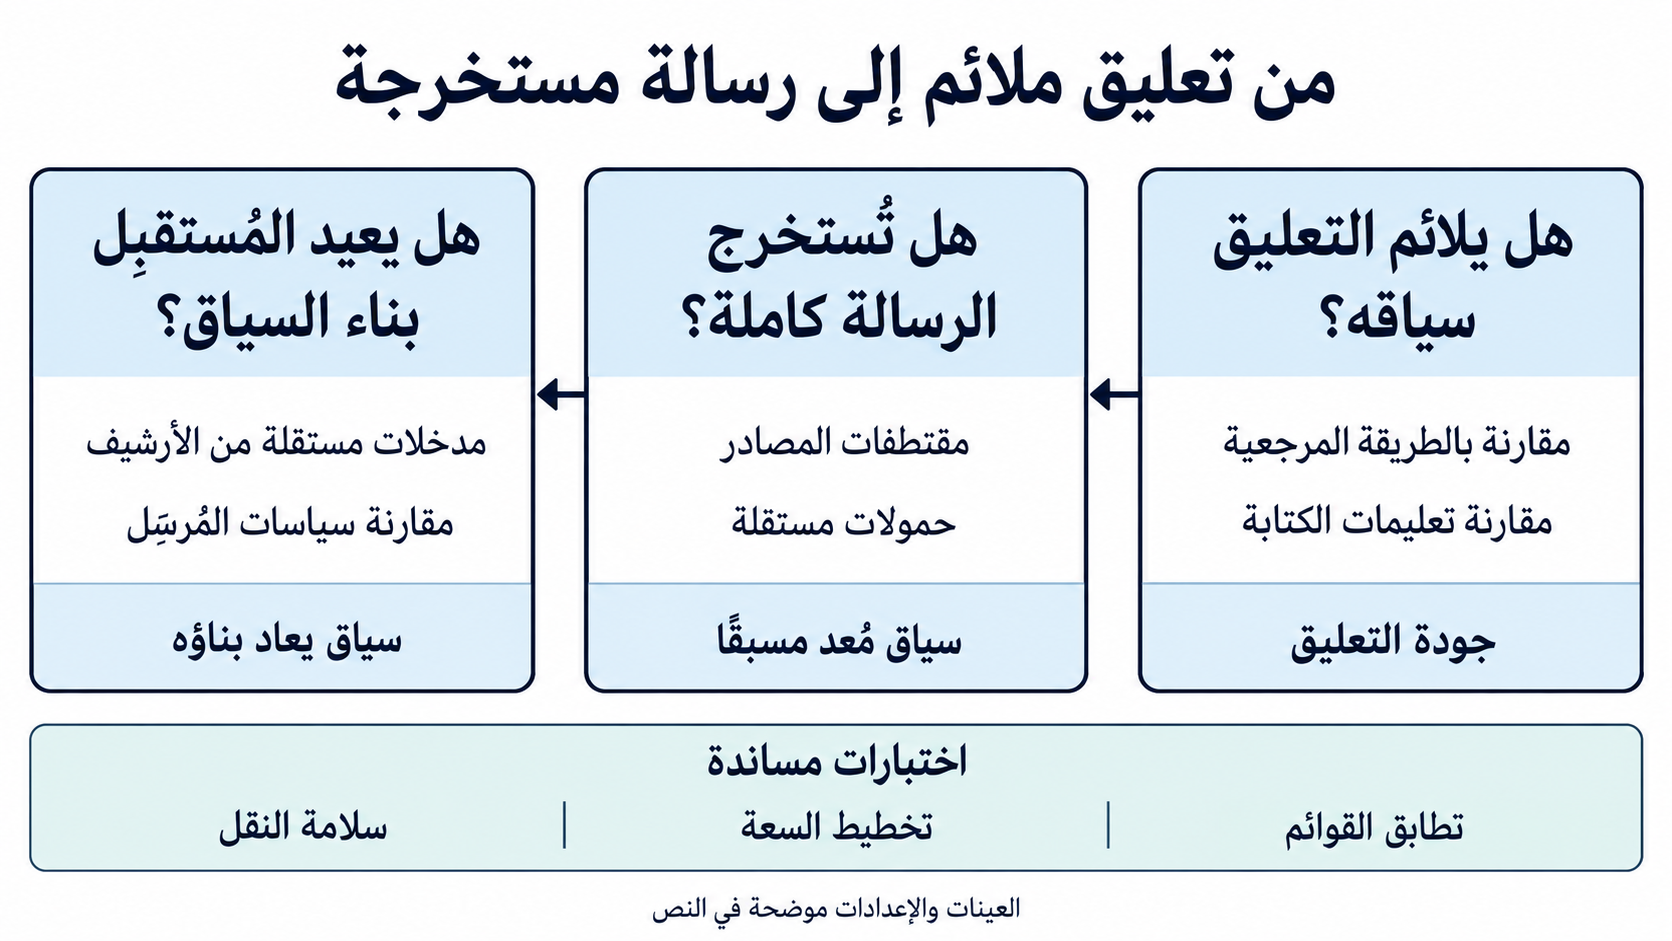
\includegraphics[width=\linewidth]{figures/evaluation_roadmap_ar.png}
\caption{تنظيم التقييم بحسب السؤال الذي تجيب عنه كل تجربة. تتطلب جودة التعليق واستخراج الرسالة كاملة وإعادة بناء السياق بصورة مستقلة أدلة مختلفة. وتساعد الاختبارات المساندة على تحديد أسباب الإخفاق، مع بقاء العينات والإعدادات خاصة بكل تجربة.}
\label{fig:evaluation-roadmap}
\end{figure}

يجمع الجدول~\ref{tab:experiment-setup} الإعدادات اللازمة لفهم هذه الانتقالات. فهو يكمل جدول اختيار البيانات وجدول النتائج: يحدد الأول مصادر العينات، ويحدد الثاني ما يقيسه كل اختبار، بينما يبين هذا الجدول أدوار النماذج وحدود محاولات التوليد وشروط الاستقبال. وتشمل المحاولات المحاولة الأولى وما يليها من إعادات؛ فالسماح بمحاولتين يعني السماح بإعادة واحدة. ويوضح القسم~\ref{sec:model-settings} الغرض من الإعدادات بجانب العمليات التي تتحكم فيها.

\begin{table}[H]
\centering\small
\caption{إعدادات المقارنات وتجارب الاستخراج الرئيسية. تخص كل مجموعة إعدادات التجربة المذكورة، ولا تمثل إعدادًا موحدًا للطريقة. ولا يكفي اسم عائلة النموذج لتحديد بيئة تنفيذه كاملة.}
\label{tab:experiment-setup}
\renewcommand{\arraystretch}{1.12}
\begin{RTL}
\begin{tabularx}{\linewidth}{|A{0.19\linewidth}|B|B|B|}
\hline
التجربة & النماذج وأدوارها & الكتابة ومحاولات التوليد & الحمولة وشروط الاستقبال \\ \hline
مقارنة الطريقتين في التجربة الأولى & لا يحدد جدول النتائج الأصلي هوية النموذج وبيئة تنفيذه تحديدًا كاملًا. & اختيار موضع الرد وفق الإعداد الأول المستخدم؛ حد أقصى قدره \NUM{32} موضوعًا. & اختيار في تعليق واحد؛ مقتطفات لـ\EN{ZLG} بحسب سعة كل عينة؛ استخراج بمساعدة سجلات المُرسِل. \\ \hline
تقييم جودة التعليقات & عائلة \EN{Qwen 3.5 9B} للتوليد لدى الطريقتين؛ و\EN{GPT-5.6 Luna} باستدلال مرتفع للتحكيم. & \EN{prompt} الكتابة الطبيعية؛ حرارة الكتابة \NUM{0.7}؛ محاولتان على الأكثر في التجربة المصدرية. & مقارنة تعليق واحد مع استخدام سجلات المُرسِل؛ خمسة معايير تحكيم على الأزواج الـ\NUM{244} نفسها. \\ \hline
مقارنة تعليمات الكتابة & لا تحدد سجلات اختيار العينة هوية نموذج التوليد كاملة؛ و\EN{GPT-5.6 Luna} باستدلال مرتفع لتمييز التعليق. & الأنماط من \EN{G0} إلى \EN{G5} ونمط جدلي؛ السياقات ومواضع الرد نفسها في \NUM{48} منشورًا. & مرشحات ذات موضوع مستهدف وأخرى ضابطة دون موضوع؛ تحقق الموضوع لدى المُرسِل، لا استخراج رسالة كاملة. \\ \hline
استخراج مقتطفات المصادر & نموذج \EN{Qwen 3.5 9B} محلي للتوليد وتحديد الموضوع. & \EN{prompt} يركز على الموضوع المختار؛ حرارة الكتابة \NUM{0.7}؛ حتى سبع محاولات لكل تعليق و\NUM{12} تعليقًا للرسالة. & مقتطفات من نصوص قاموس الضغط؛ قوائم مُعدة وترتيب تعليقات موفر للمُستقبِل. \\ \hline
التطوير بحمولات مستقلة & \EN{GPT-6 Luna} باستدلال منخفض عبر سطر الأوامر؛ بحث دلالي باستخدام \EN{MiniLM}. & محاولتان على الأكثر لكل تعليق و\NUM{20} تعليقًا للرسالة؛ لا تتيح الأداة ضبط الحرارة. & رسائل مستقلة من ثمانية بايتات؛ سياق مُعد مسبقًا؛ يحدد المُستقبِل الموضوع باستخدام البحث المعتاد. \\ \hline
إعادة البناء من الأرشيف & \EN{Qwen 3.5 9B} محلي؛ و\EN{GPT-OSS 20B} لفحص جودة الكتابة في مقارنة السياسات. & مقارنة الكتابة المركزة على الموضوع مع \EN{G5} بمحاولتين، ثم مقارنة محاولتين بسبع. حرارة الكتابة \NUM{0.7} وتحديد الموضوع \NUM{0}؛ حتى \NUM{20} تعليقًا في مقارنة السياسات. & رسائل مستقلة من ثمانية بايتات؛ قوائم مستخرجة من المحادثة فقط؛ يجلب كل طرف مدخلاته من الأرشيف بصورة مستقلة. \\ \hline
\end{tabularx}
\end{RTL}
\end{table}

تختلف بيئة النماذج المحلية عن مسار سطر الأوامر بحسب التجربة. يسجل ملف إعداد تجربة مقتطفات المصادر بطاقة \EN{NVIDIA GeForce RTX 5060 Ti} بذاكرة تقارب \NUM{16} غيغابايت. وتحدد سجلات مقارنة سياسات الأرشيف نموذج \EN{Qwen} المقدم عبر \EN{LM Studio} بضغط عددي من نوع \EN{Q4\_K\_M} وسياق محمل يبلغ \NUM{16384} رمزًا؛ وهذه مواصفات تلك المقارنة تحديدًا. أما التطبيق الرسمي لـ\EN{ZLG}، فيستخدم بيئة خاصة تتيح احتمالات الرموز. ولا يعني اشتراك الطريقتين في عائلة \EN{Qwen} في مقارنة الجودة تطابق التنفيذ أو الكلفة الحسابية. وفي تجربة سطر الأوامر، يُطلب اسم النموذج ومستوى الاستدلال دون إتاحة ضبط الحرارة؛ لذلك لا ننسب إليها إعدادات النموذج المحلي الحالية.

يجب كذلك تحديد تعليمات الكتابة التي استُخدمت. تعتمد تجربة الجودة حزمة \EN{prompt} الكتابة الطبيعية، بينما تستخدم تجربة المقتطفات والطريقة الأساسية في الأرشيف حزمة تركز الرد على الموضوع المختار ضمن سياق التعليق الأب. ويضيف \EN{G5} تعليمات الرد الحواري وثلاثة أمثلة بشرية ثابتة، كما يوضح القسم~\ref{sec:prompt-ablation}. يشرح الفصل~\ref{sec:methodology} بناء الموضوعات، ويشرح القسم~\ref{sec:receiver-operation} تحديدها لدى المُستقبِل، ويورد الملحق~\ref{app:judge-material} نصوص الـ\EN{prompts} المستخدمة في تحكيم الجودة. أما محكّم مقارنة الإيجاز، فيستخدم \EN{GPT-OSS 20B} بحرارة صفر ويعرض ترتيبَي المرشحين، وفق القسم~\ref{sec:fresh-archive}. تخص هذه الإعدادات المحكّم ولا تصف نموذج كتابة التعليقات.

تدعم اختبارات إعداد القوائم، وتجربة الحد البالغ ثمانية تعليقات، وفحص سلسلة الردود، واختبارات النقل دون النموذج أجزاء محددة من هذا المسار. وتبقى مدخلاتها وحدودها موضحة في الجدول~\ref{tab:evidence-levels} وفي مواضع شرحها، ولا تُنسب إليها إعدادات تجربة مجاورة. ونربط الكلفة بالعملية التي قِيست: جمع المصادر وإعدادها، أو توليد المرشحات والتحقق منها، أو الاختيار بين الردود المقبولة، أو استقبال التعليقات. فاستخدام مدخلات مُعدة مسبقًا يستثني كلفة جمعها من القياس، كما أن مجموع مدد استدعاء النموذج لا يساوي بالضرورة الزمن الفعلي للعملية كاملة.
